\chapter{Namespaces}
\section{Why we need Namespaces}
\subsection{Namespaces}
\begin{itemize}
\item If in the same document two or more XML languages are used, we risk to get name clashes of elements or attributes.
\item Namespaces are used to indicated which elements and attributes in the document belong to the same language.
\item Programmers are pretty familiar with this sort of problem: C\# also has namespaces; Java prefers the name package.
\end{itemize}

\section{Two XML Languages in one document}
\begin{lstlisting}[language=XML, caption={Where does the error occur?}]
<bond_movies>
...
<movie number="_20">
<title>Die another day</title>
<bond>Pierce Brosnan</bond>
<bond_girl>Halle Berry</bond_girl>
<regie>Lee Tamahori</regie>
<year>2002</year>
<plot>
<html>
<head><title>Die Another Day, 2002</title></head>
<body>James Bond infiltrates a North Korean military base, where Colonel Tan-Sun Moon is illegally trading African <i>conflict diamonds</i> for weaponry. After Moon's assistant Zao discovers Bond is a British agent, the colonel escapes in a hovercraft. Bond distracts the soldiers with an explosion, in which Zao's face is disfigured by diamond fragments. Bond pursues Moon in a second hovercraft. During the chase, Moon's hovercraft plunges down a waterfall, apparently killing him. Bond is captured by North Korean soldiers and imprisoned by the Colonel's father, General Moon. After 14 months of captivity and torture, Bond is traded for Zao in a prisoner exchange. He is sedated and taken to meet <b>M</b>, who informs him that his status as a <b>00 Agent</b> is suspended due to her belief that he may have leaked information under duress. Still bitter over Zao's release, Bond decides to complete his mission by evading MI6's security and travelling to Hong Kong, where he learns from his contact in the Chinese government that Zao was sighted in Cuba ...</body></html></plot> </movie>
...
</bond_movies>
\end{lstlisting}

\section{Default Namespace Example}

\begin{lstlisting}[language=XML, caption={Default Namespace}]
<?xml version="1.0" encoding="UTF-8"?> <html>
<head>
<title>XHTML and SVG in the same Document</title>
  </head>
  <body>
    <h1>An image ...</h1>
<svg xmlns="http://www.w3.org/2000/svg"> <g>
<title>Do I appear as a tooltip ?</title>
<rect x="10" y="10" width="200" height="50" style="fill:blue"/> </g>
</svg>
  </body>
</html>
\end{lstlisting}
The element \code{<svg>} and every element contained (aka. children) now belong to the given namespace. But \textbf{the attributes do not} !Attributes are not children of any element.

\begin{itemize}
\item In contrast, attributes do not automatically belong to default namespaces, e.g. the attribute width is not in the given namespace.
\item Attributes are always associated with elements. They cannot stand alone. If the element belongs to a namespace, the attribute is already uniquely identifiable.
\item If attributes shall belong to a namespace, they must be assigned explicitly using a prefix (next slide).
\item In most cases, there is no need for attributes to belong to namespaces. An exception are XLink attributes.
\item We may want to have an element that belongs to namespace 1 with an attribute that belongs to namespace 2. Hence, attributes must not automatically belong to an element’s namespace.
\end{itemize}

\section{Explicit Namespace with Prefix}
\begin{lstlisting}[language=XML, caption={Default Namespace}]
<?xml version="1.0" encoding="UTF-8"?> 
<html>
<head>
	<title>XHTML and SVG in the same Document</title>
  </head>
  <body>
	<h1>An image ...</h1>
	<svg xmlns:hr="http://www.w3.org/2000/svg">
		<g>
			<title>Do I appear as a tooltip ?</title>
			<rect x="10" y="10" width="200" height="50" style="fill:blue"/>
		</g> 
	</svg>
</body>
</html>
\end{lstlisting}

With a prefix we identify the namespace. It is no more a default namespace and no element (not even <svg>) belongs to this
namespace yet.

\subsection{Second approach}
\begin{lstlisting}[language=XML, caption={Default Namespace}]
<?xml version="1.0" encoding="UTF-8"?> 
<html>
	<head>
		<title>XHTML and SVG in the same Document</title>
	</head>
	<body>
   		<h1>An image ...</h1>
		<hr:svg xmlns:hr="http://www.w3.org/2000/svg"> 
			<hr:g>
				<hr:title>Do I appear as a tooltip ?</hr:title>
				<hr:rect x="10" y="10" width="200" height="50" style="fill:blue"/> 
			</hr:g>
		</hr:svg>
  	</body>
</html>
\end{lstlisting}
This reproduces the situation we had with the default namespace. The element \code{<svg>} and all sub-elements now belong to the
namespace. However, the attributes still do not.\\
The attributes could be put into the namespace by simply writing \code{hr:} in front of them, but there is often no need for that.

\subsubsection{Some W3C namespaces}
\begin{figure}[h!]
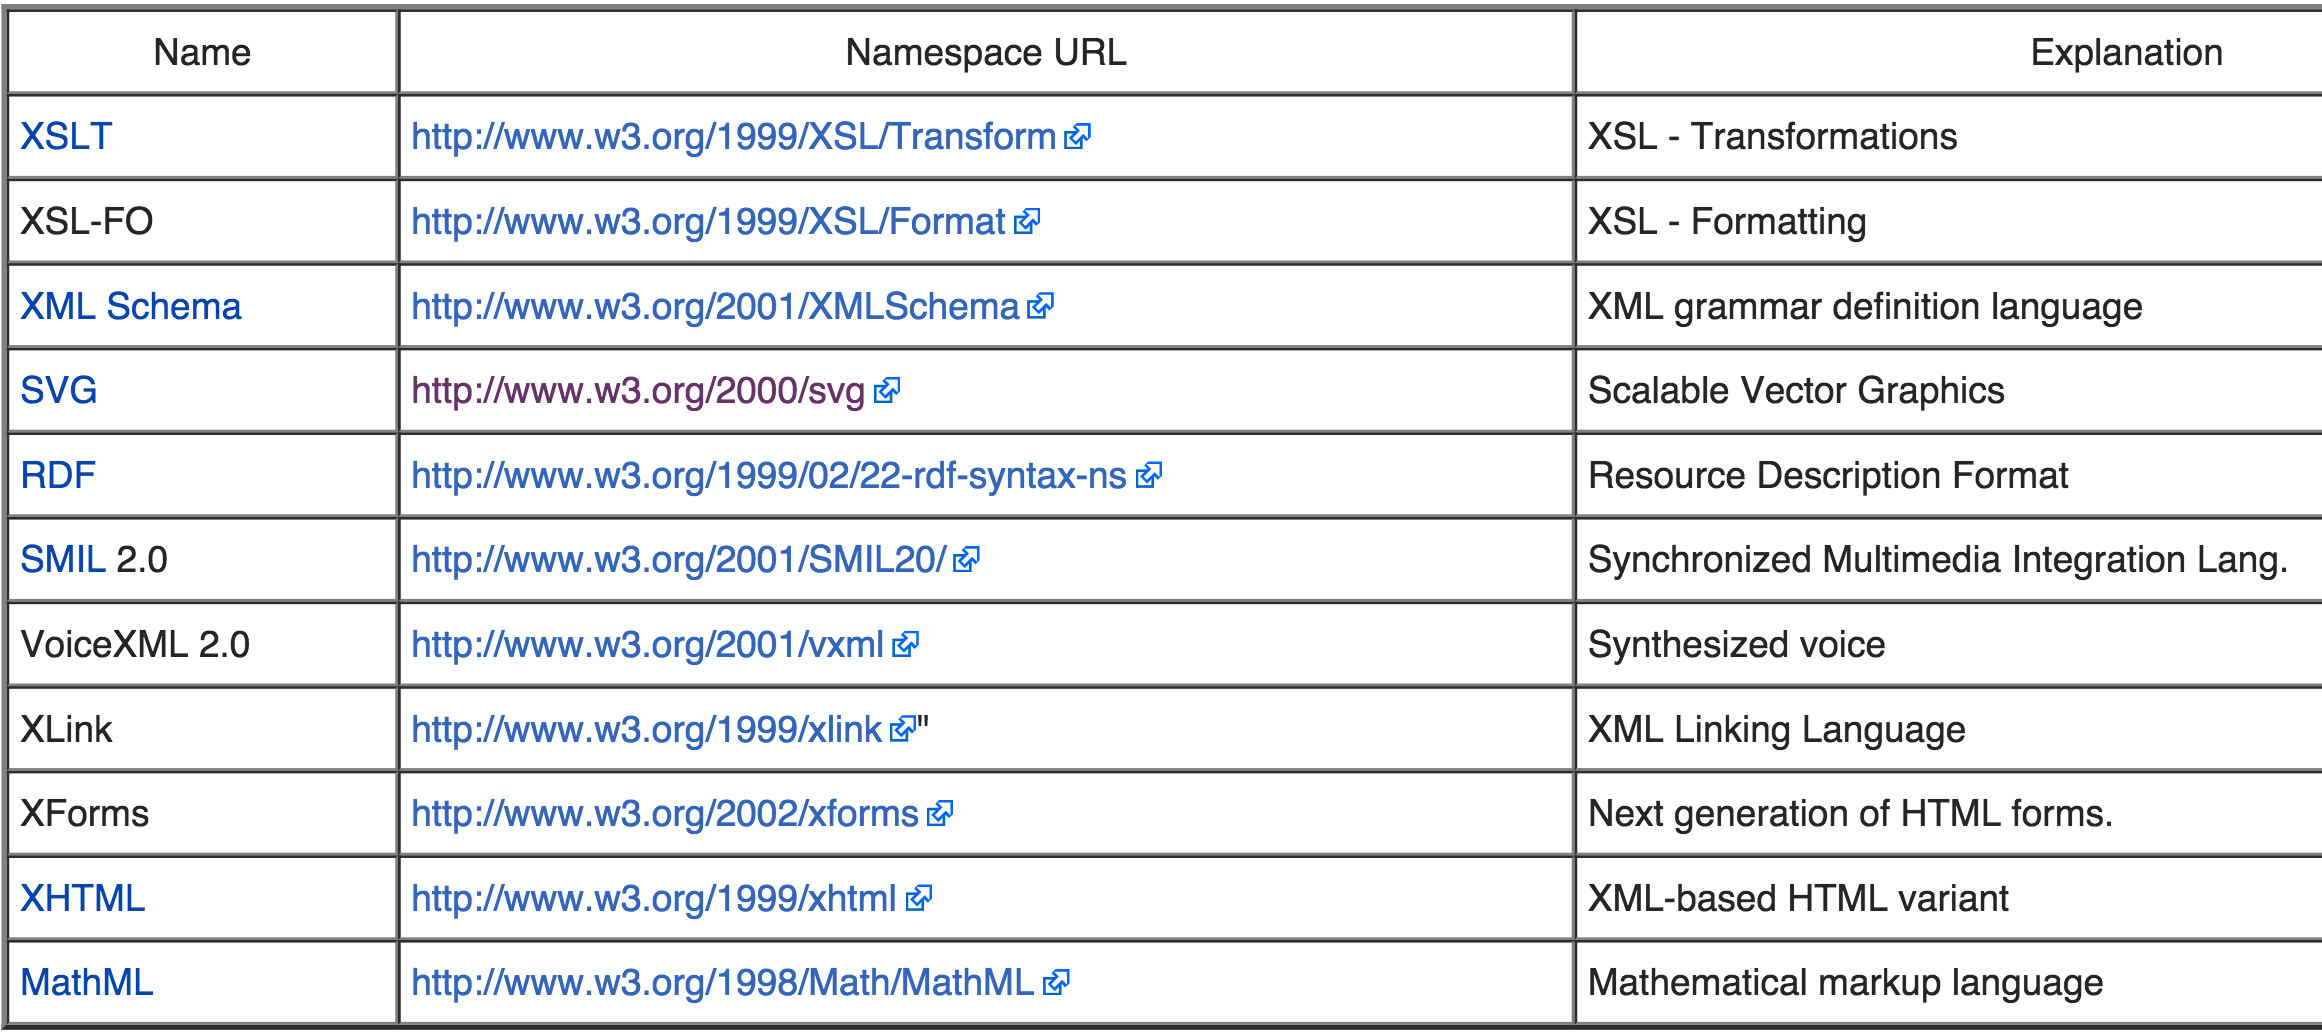
\includegraphics[width=\textwidth]{fig/W3CNamespaces.png}
\end{figure}

\section{Common difficulties with namespaces}
\begin{itemize}
\item Namespaces are case-sensitive, be consistent when inventing them.
\item Namespaces look like attributes – they are not. They will not show up in attribute lists obtained from parsers for example.
\item Comments do not have namespaces.
\item Namespace declarations must come either on the element that uses it or higher in the tree. Attention: on the same tree-level but earlier in the file does not work.
\item To avoid this difficulty, it is common to declare namespaces in the root and to use prefixes when necessary. But you don‘t have to.
\end{itemize}

\section{Control Questions A}
\begin{enumerate}
\item Name two* reasons why namespaces are important.\\
So that the processor knows to which Namespace a tag corresponds. Damit wir XML-Dokumente validieren (an ein Schema binden) können.
\item Explain the difference between URLs, URNs and URIs.\\
\begin{center}
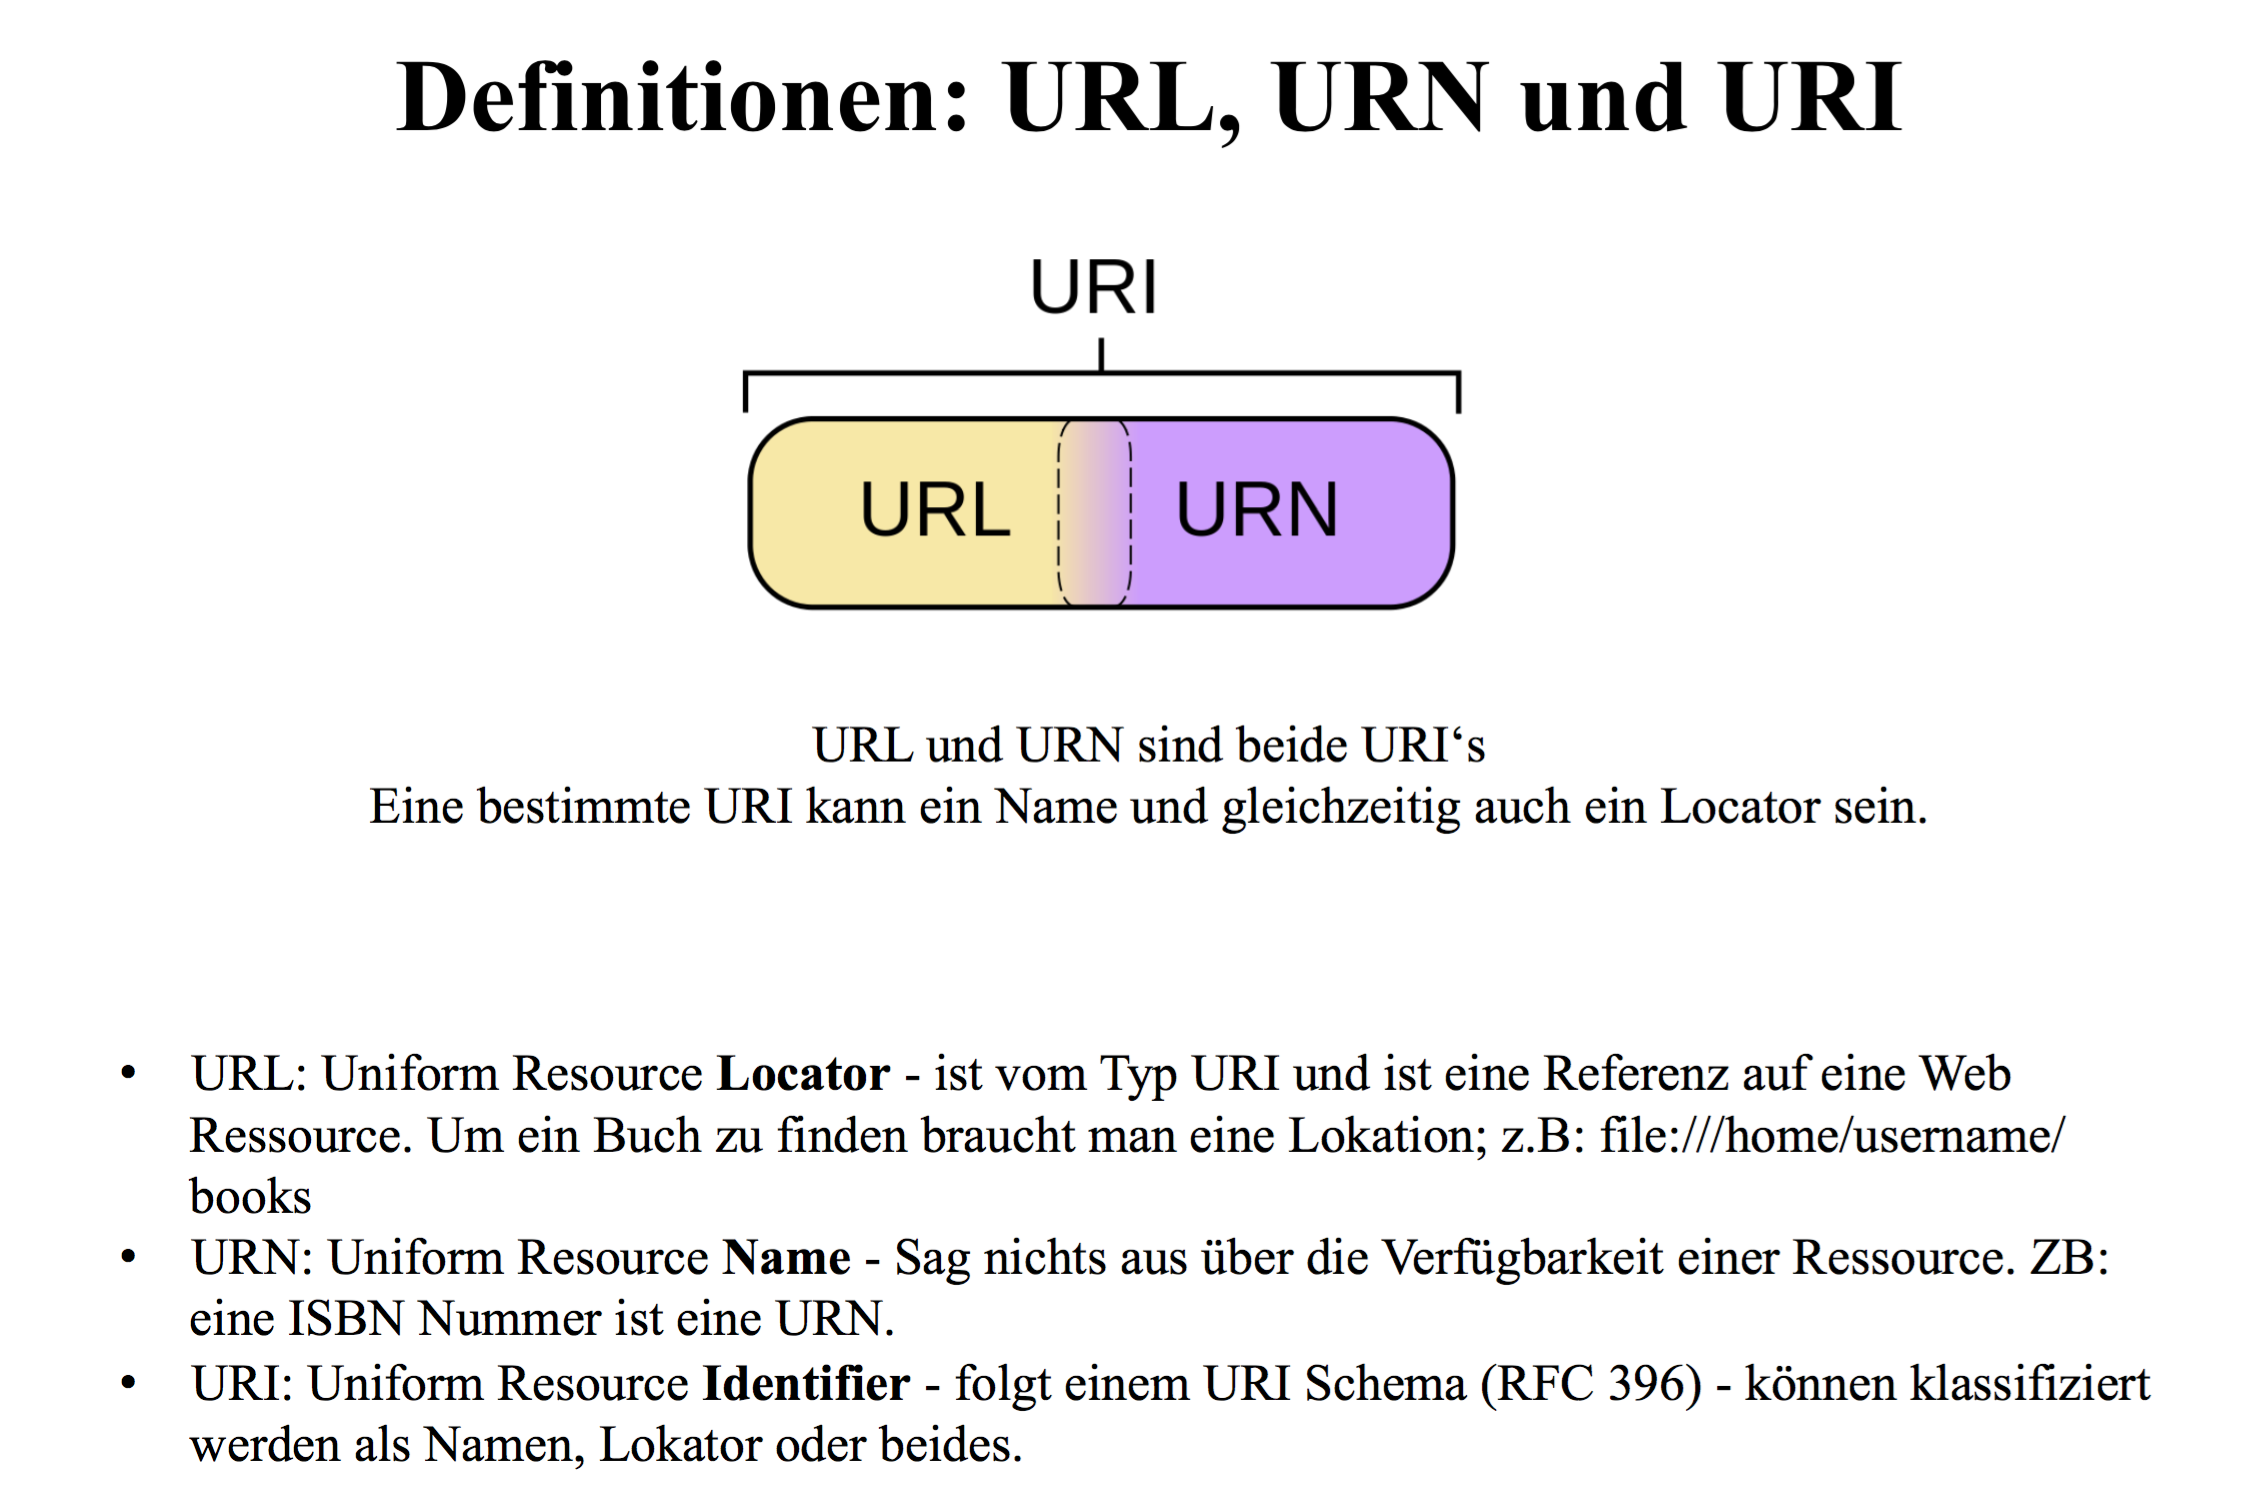
\includegraphics[width=0.7\textwidth]{fig/URI.png}
\end{center}
\item Explain the difference between a default and a prefix namespace.\\
Default Namespace inkludiert alle untergeordneten Tags in diesen Namespace, ein Prefix Namespace muss bei jedem Tag den Namespace angeben.
\item In which regard are attributes special with respect to namespaces ?\\
Attribute nehmen nicht automatisch den Namespace des Default Namespaces an, sondern müssen mit Präfix deklariert werden.
\item What is the XML namespace and why is it special ?\\
Der XML Namespace kann immer verwendet werden (ist automatisch referenziert).
\item Typical exam question on namespaces:
\begin{itemize}
\item Debug an XML document with incorrectly used namespaces
\end{itemize}
\end{enumerate}
